% =====================================================================
% Conference paper in ieeeconf format, targeting ECC. 6-page limit.
%
% FRAMING (settled): the paper's object is the LIMIT CYCLE of fixed-step
% and accelerated SPIN tuning. The triple point is the tool that locates
% the cycle's center; the regularized index is the tool that makes the
% analysis well posed. Neither appears in the title.
%
% Numbers policy: all from verified follow-up runs. TODO-REGEN entries
% need regeneration before submission; TODO marks editorial placeholders.
% =====================================================================
\documentclass[letterpaper, 10pt, conference, twocolumn]{ieeeconf}

\usepackage{amsmath,amssymb,amsthm}
\usepackage{graphicx}
\usepackage{booktabs}

\newtheorem{proposition}{Proposition}
\newtheorem{corollary}{Corollary}
\newtheorem{lemma}{Lemma}
\newtheorem{observation}{Observation}
\newtheorem{remark}{Remark}

\newcommand{\Nbar}{\bar{N}}
\newcommand{\Neps}{N_{\varepsilon}}

% Paper title
\title{Limit Cycles of Model-Free PID Tuning by Step-Response Inspection}

% Author names and affiliations
\author{Daniel Pachner$^{1}$, Pavel Otta$^{1}$, Ji\v{r}\'{\i} Dost\'al$^{1}$
and Vladim\'{\i}r Havlena$^{2}$%
\thanks{$^{1}$University Centre for Energy Efficient Buildings (UCEEB),
Czech Technical University in Prague, Bu\v{s}t\v{e}hrad, Czech Republic.
Corresponding author: \texttt{pavel.otta@cvut.cz}}%
\thanks{$^{2}$Department of Control Engineering, Faculty of Electrical
Engineering, Czech Technical University in Prague, Prague, Czech Republic.}%
}

\begin{document}

\maketitle

\begin{abstract}
In a companion paper we introduced SPIN, a model-free PID tuning method
that inspects three phase portraits of the closed-loop step response,
counts a turn index in each, and adjusts the gains by a fixed table of
four moves with a constant step size. In practice the iteration does not
converge to a point: it settles into a small periodic orbit. This paper
investigates that limit cycle. We show that the cycle is not an artifact
but a structural feature of the rule: in log-gain coordinates the four
moves admit a unique vanishing convex combination, which forces the
cycle to orbit the \emph{triple point} --- the gain vector at which all
three turn indices sit exactly on their thresholds --- with move
frequencies $(\tfrac18, \tfrac12, \tfrac14, \tfrac18)$ fixed by the
balance. Measured frequencies match this prediction to three decimal
places. The same balance taken over the integers forces a minimal period
of eight, and the terminal orbit realizes it as a binary odometer on the
corners of a cube of side $\log\gamma$ centred on the triple point.
Making these statements well posed requires replacing the published
integer count by an $\varepsilon$-regularized winding integral, which we
introduce as an analysis tool. The theory directly supports practical
tuning. Because the cycle is an axis-aligned cube, a fixed step $\beta$
leaves every gain within the factor $(1-\beta)^{-1/2}$ of the
plant-determined target, so a per-gain tolerance $\rho$ is met by
choosing $\beta \le 1-\rho^{-2}$; the companion paper's default
$\beta = 0.1$ certifies $5.4\,\%$ per gain. An accelerated schedule that
halves the step whenever every band has reversed shrinks the cube
geometrically, reaching $10^{-4}$ accuracy in under a hundred
iterations.
\end{abstract}

\begin{IEEEkeywords}
PID control, model-free tuning, limit cycles, switched systems,
winding number
\end{IEEEkeywords}

% =====================================================================
\section{Introduction}
\label{sec:intro}

Most PID tuning methods fit a model first and compute gains second
\cite{ZN1942,AstromHagglund2004}. In a companion paper \cite{Paper1} we took
a different route: tune directly from what the step response \emph{looks like}.
The method, SPIN (Step-response Phase-portrait INspection), draws three phase
portraits from one closed-loop step response, counts how many times each curve
turns around the origin --- the \emph{turn index} $N_k$ of band $k$ --- and
compares each count to a fixed threshold. A table of four moves, the
\emph{triangular rule}, then scales the gains up or down by a constant factor.
No plant model is identified at any point.

The companion paper demonstrates that the rule detunes aggressive gains,
recovers from failed loops, and lands in a feasible region on a battery of
standard plants. It also shows, without explaining, a characteristic terminal
behavior: instead of converging to a point, every successful run ends in a
small periodic orbit in gain space. This limit cycle is the object of the
present paper. Three questions organize the investigation. Where is the cycle
--- what point does it orbit, and is that point determined by the plant or by
the algorithm's history? What is its shape and size --- which moves occur, in
what proportion, how short can a cycle be, and can the step size be chosen to
meet a stated gain tolerance? And can the cycle be shrunk --- is there a
practical accelerated schedule whose accuracy the theory can guarantee rather
than merely observe?

Our answers: the cycle orbits a single plant-determined point, the
\emph{triple point}, at which all three turn indices sit exactly on their
thresholds (Section~\ref{sec:cycle}); its move frequencies and its minimal
period of eight are forced by a unique convex balance of the four moves, its
realization is a binary odometer on the corners of a cube of side
$\log\gamma$, and this geometry yields a closed-form rule for choosing the
step from a per-gain tolerance (Sections~\ref{sec:cycle}
and~\ref{sec:size}); and a reversal-triggered halving schedule shrinks the
cycle geometrically to $10^{-4}$ accuracy in under a hundred iterations
(Section~\ref{sec:accel}). Along the way we need one technical repair: the
published turn index is an integer count, discontinuous in the gains, under
which the cycle's center is not even well defined. Section~\ref{sec:index}
introduces an $\varepsilon$-regularized winding integral that fixes this. We
stress its role: it is an instrument of the analysis, not a change to the
method --- every sign comparison the published rule makes is unchanged.

It is worth stating what kind of object we are analyzing. Iterative model-free
tuning is not new: iterative feedback tuning estimates the gradient of a
performance criterion from closed-loop experiments and converges, with an
appropriately shrinking step, to a local minimum of that criterion
\cite{Hjalmarsson1998}; extremum seeking does the same with sinusoidal probing
\cite{Killingsworth2006}. The triangular rule is different in kind. It is a
\emph{sign-based} update with no cost function and no gradient, so its natural
terminal object is not a stationary point but a limit cycle of a switched
system --- and limit cycles of switched systems are exactly what the tools of
averaged (Filippov) dynamics are made for \cite{Filippov1988}.

% =====================================================================
\section{The Rule as a Switched System}
\label{sec:rule}

We recall only what is needed; the companion paper \cite{Paper1} defines the
portraits, the index, and the rule in full. One closed-loop step experiment
yields three curves (band $0$, $1$, $2$), and for each curve a turn index
$N_k \ge 0$ measuring how far the curve winds around the origin of its
portrait. Each band has a fixed threshold:
\begin{equation}
\Nbar = (\Nbar_0, \Nbar_1, \Nbar_2) = (0.5,\; 0.75,\; 1.0).
\label{eq:thresholds}
\end{equation}

The triangular rule reads the three comparisons $N_k \gtrless \Nbar_k$ and
applies one of four moves to the gain vector. Following \cite{Paper1} we
order the gains by the band each channel dominates,
$K^{(0)} = K_i$, $K^{(1)} = K_p$, $K^{(2)} = K_d$, so that $N_k$ is the index
pointing at $K^{(k)}$. If all
three bands are below threshold, all gains are scaled up; otherwise the lowest
offending band is cut by scaling gains down in a band-specific pattern. Every
move multiplies each gain by $\gamma^{\pm 1}$ or leaves it alone, where
$\gamma = 1/(1-\beta)$ and $\beta$ is the step size (default $\beta = 0.1$,
so $\gamma \approx 1.111$). Multipliers are clipped to a box, here
$[0.01, 10]$.

Throughout we assume the step response is measured without output noise, so
that each turn index is a deterministic function of the gains. The stochastic
case, in which the three comparisons become random near the target, is treated
in follow-up work; the deterministic characterization below is its zero-noise
limit, and Proposition~\ref{prop:unique} records a combinatorial property of
the move table that bears on it.

In log coordinates $\theta = (\log K_i, \log K_p, \log K_d)$ --- band order,
\emph{not} the customary PID order --- the four moves become translations by
$h = \log\gamma$:
\begin{equation}
\begin{aligned}
e   &= (+1, +1, +1) &\text{(expand),}\\
d_0 &= (-1, \phantom{+}0, \phantom{+}0) &\text{(cut band 0),}\\
d_1 &= (+1, -1, \phantom{+}0) &\text{(cut band 1),}\\
d_2 &= (+1, +1, -1) &\text{(cut band 2),}
\end{aligned}
\label{eq:moves}
\end{equation}
each scaled by $h$. The iteration is a switched dynamical system: a partition
of gain space into four regions (determined by the signs of $N_k(\theta) -
\Nbar_k$), with a constant velocity assigned to each region. Because the
velocity is constant inside each region, the state cannot rest anywhere: a
bounded trajectory must forever cross between regions. The terminal behavior
of the rule is therefore necessarily a cycle, and the analysis reduces to two
questions --- where the regions meet, and how the crossing pattern organizes
itself there.

% =====================================================================
\section{The Limit Cycle and Its Center}
\label{sec:cycle}

Suppose a trajectory stays bounded and does not drift. Over a long window,
each move $v \in \{e, d_0, d_1, d_2\}$ is applied some fraction $w_v \ge 0$ of
the time, with $\sum_v w_v = 1$. Non-drifting requires the average
displacement $h \sum_v w_v v$ to vanish.

\begin{proposition}[Unique Balance]
\label{prop:balance}
The only convex combination of the moves \eqref{eq:moves} that vanishes is
\begin{equation}
\tfrac{1}{8}\, e + \tfrac{1}{2}\, d_0 + \tfrac{1}{4}\, d_1
+ \tfrac{1}{8}\, d_2 = 0.
\label{eq:weights}
\end{equation}
\end{proposition}

All four weights are strictly positive, which pins down the cycle completely
in two respects.

\begin{corollary}[Center of the Cycle]
\label{cor:triple}
A bounded, non-drifting trajectory must apply all four moves with the
frequencies \eqref{eq:weights}, and can therefore only orbit a point
$\theta^*$ where all three switching surfaces meet:
\begin{equation}
N_k(\theta^*) = \Nbar_k, \qquad k = 0, 1, 2.
\label{eq:triplepoint}
\end{equation}
We call $\theta^*$ the \emph{triple point}. It is determined by the plant and
the thresholds alone --- not by the step size, the starting gains, or the
history of the run.
\end{corollary}

The same elimination, run over the integers, bounds the cycle length from
below: there is no shorter limit cycle than the one observed.

\begin{corollary}[Minimal Period]
\label{cor:period}
Any exactly closed orbit applies the moves an integer number of times
$(n_e, n_{d_0}, n_{d_1}, n_{d_2})$ with $\sum_v n_v\, v = 0$, which forces
$(n_e, n_{d_0}, n_{d_1}, n_{d_2}) = n_e \cdot (1, 4, 2, 1)$. Every closed
orbit therefore has length a multiple of $8$; the shortest possible cycle
has length exactly $8$, and no closed orbit can avoid any of the four moves.
\end{corollary}

The corollaries make three testable predictions: the location of the cycle,
its move frequencies, and its minimal length. All hold with striking
precision. On plants P1, P3, P4 of the companion battery, long constant-step
runs settle into a period-8 orbit around a single point, and the measured
duty cycle of the four moves matches
$(\tfrac18, \tfrac12, \tfrac14, \tfrac18)$ to three decimal places, at both
$\beta = 0.10$ and $\beta = 0.03$ (Table~\ref{tab:duty}).

\begin{observation}[Odometer Orbit]
\label{obs:ruler}
On all interior-target plants the terminal orbit realizes the minimal
period~$8$ with the moves in a fixed ``ruler'' ordering,
$d_0\, d_1\, d_0\, d_2\, d_0\, d_1\, d_0\, e$. Accumulating these moves, the
eight visited points are exactly the corners of a cube of side
$h = \log\gamma$ centred on $\theta^*$, traversed in binary counting
order: $\log K_i$ acts as the least significant bit, $\log K_p$ and
$\log K_d$ as the higher bits, and $e$ as the carry that resets the counter
(Fig.~\ref{fig:cycle}). In particular every point of the orbit lies at the
same distance $\tfrac{\sqrt{3}}{2}\, h$ from the centre.
\end{observation}

Corollaries~\ref{cor:triple} and~\ref{cor:period} force the frequencies, the
length, and (given the ordering) the cube geometry of
Observation~\ref{obs:ruler}; what remains a measurement is the ruler
\emph{ordering} itself --- other orderings of the same move multiset would
close geometrically, and it is the switching law that selects this one.
Proving that selection is part of the program of
Section~\ref{sec:structure}.

\begin{figure}[t]
\centering
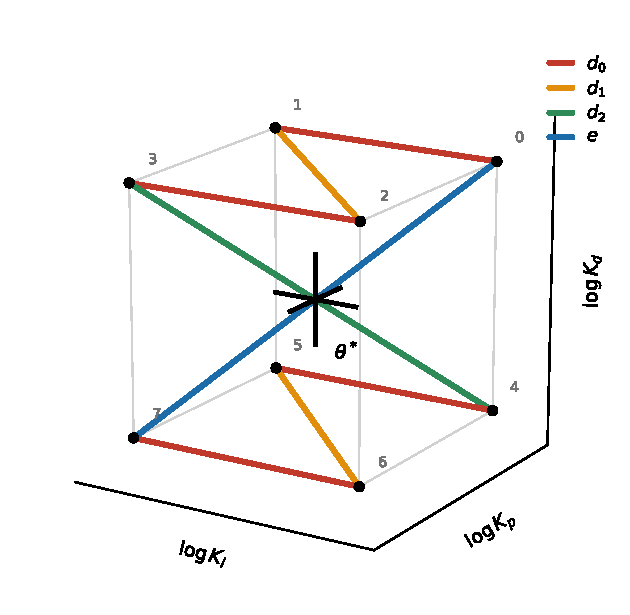
\includegraphics[width=0.9\linewidth]{fig_limit_cycle}
\caption{The limit cycle in log-gain space. One period visits the eight
corners of a cube of side $h = \log\gamma$ centred on the triple point
$\theta^*$ (black cross), in binary counting order (vertex labels); the
moves $d_0, d_1, d_2, e$ act as bit toggles and carries. The two space
diagonals ($e$, $d_2$) pass through the centre.
% NOTE: schematic drawn from the ruler ordering implied by the measured
% duty cycle; verify against a recorded terminal orbit (TODO-REGEN) and
% ideally replace/accompany with the measured orbit on P1.
}
\label{fig:cycle}
\end{figure}

\begin{remark}[Reduced-Order Hierarchy]
\label{rem:hierarchy}
The argument is not specific to three gains. For an $n$-gain triangular rule
with the analogous staircase moves ($e$ all $+1$; $d_k$ equal to $+1$ on the
first $k$ coordinates, $-1$ on coordinate $k$, zero after), the unique
balance has weights $w_{d_k} = 2^{-(k+1)}$ and $w_e = 2^{-n}$, the minimal
period is $2^n$, and the minimal orbit is a binary counter on the corners of
the $n$-cube: a two-point segment for pure integral tuning ($n{=}1$,
weights $\tfrac12, \tfrac12$), a square for PI ($n{=}2$, weights
$\tfrac14, \tfrac12, \tfrac14$), the cube of Fig.~\ref{fig:cycle} for PID
(Fig.~\ref{fig:hierarchy}).
% NOTE: for n=1,2 this presumes the rule keeps the same staircase move
% pattern; the companion paper defines the rule for PID only, so verify
% the reduced-order move sets against the implementation before relying
% on this remark quantitatively.
\end{remark}

\begin{figure}[t]
\centering
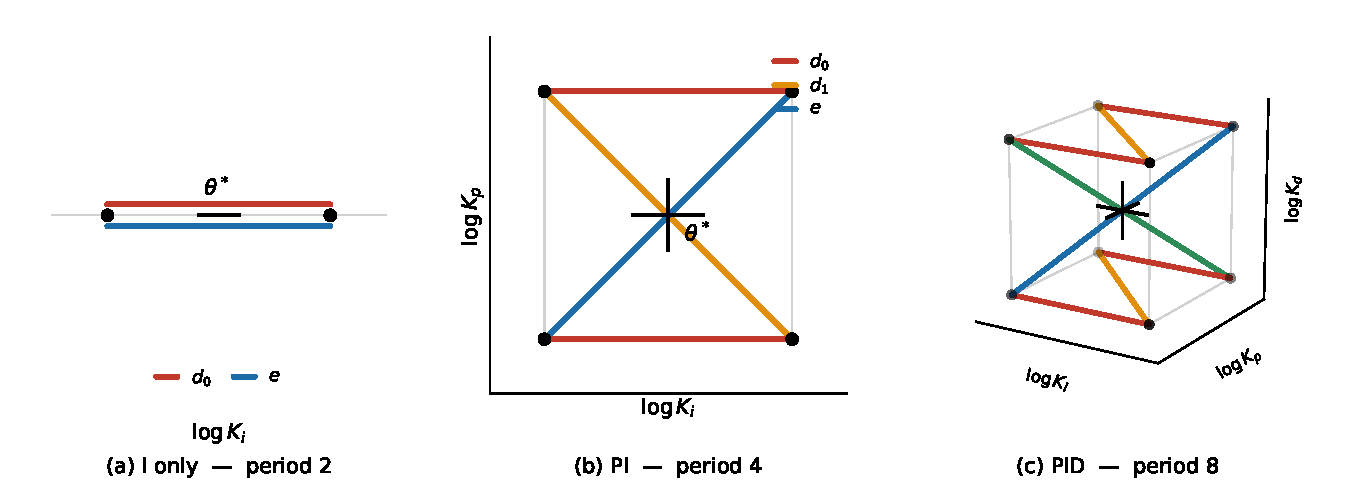
\includegraphics[width=\linewidth]{fig_limit_cycle_hierarchy}
\caption{The limit-cycle hierarchy of Remark~\ref{rem:hierarchy}: minimal
orbits for I-only ($n{=}1$, period 2), PI ($n{=}2$, period 4), and PID
($n{=}3$, period 8) tuning are binary counters on the corners of the
$n$-cube of side $h$, centred on the corresponding threshold point
$\theta^*$.}
\label{fig:hierarchy}
\end{figure}

\begin{proposition}[The Move Table is Forced]
\label{prop:unique}
Fix the priority order of the rule. Among move tables in which
(i) every entry lies in $\{-1, 0, +1\}$, so that each gain is multiplied by
$\gamma^{\pm 1}$ or left alone; (ii) $e = (1, \dots, 1)$; and (iii) each
cut $d_k$ decreases its own gain, $d_k[k] = -1$; the staircase table
\eqref{eq:moves} is the \emph{unique} one whose balance weights
\eqref{eq:weights} coincide with the branch frequencies of the priority
logic.
\end{proposition}

\begin{proof}
Counting sign patterns, the priority logic selects $e$ on $1$ of the $2^n$
patterns and $d_k$ on $2^{\,n-k-1}$ of them, so matching requires
$e + \sum_k 2^{\,n-k-1} d_k = 0$. Coordinate $j$ of this reads
$\sum_k 2^{\,n-k-1} d_k[j] = -1$: a signed-binary representation of $-1$ with
digits in $\{-1,0,1\}$. Exactly $n$ such representations exist, indexed by the
position $m$ of the single $-1$ digit, namely $d_m[j] = -1$, $d_k[j] = +1$
for $k > m$ and $0$ for $k < m$. Hypothesis (iii) forces $m = j$, giving
$d_k[j] = +1$ for $j < k$, $-1$ for $j = k$, and $0$ for $j > k$ --- the
table \eqref{eq:moves}.
\end{proof}

Both hypotheses are sharp: dropping (iii) admits $n^n$ matching tables, and
relaxing (i) to entries in $\{-2, \dots, 2\}$ admits six for $n = 3$.
The rule's triangular shape is therefore not a design choice but the only
shape reconciling the selection logic with the balance geometry, and the
balance weights are powers of two precisely because the selection tree is
binary.

Two consequences are worth recording. First, matching forces a favourable
pairing: $\lVert d_k \rVert = \sqrt{k+1}$ while $d_k$ fires with frequency
$2^{-(k+1)}$, so the most frequent move is always the gentlest and the
expected displacement per iteration is only $1.287\,h$, against $\sqrt{3}\,h$
for the largest move. Second, the matching has a reading under measurement
noise: if the comparisons are corrupted until their signs carry no
information, the moves fire at the branch frequencies, which are the balance
weights, so the expected displacement vanishes and the iteration holds
position at $\theta^*$ instead of drifting. This is a statement about the
move table, proved here combinatorially; a stochastic treatment, including
the correlated-noise regime in which the argument no longer applies, is left
to follow-up work.

\begin{table}[t]
\small
\centering
\caption{Measured duty cycle of the terminal orbit vs.\ the prediction of
Corollary~\ref{cor:triple}.
% TODO-REGEN: values from code/asymptotics/duty_cycle.py; matched
% to three decimals on P1, P3, P4 at both step sizes.
}
\label{tab:duty}
\begin{tabular}{lcccc}
\toprule
 & $w_e$ & $w_{d_0}$ & $w_{d_1}$ & $w_{d_2}$ \\
\midrule
Predicted & $0.125$ & $0.500$ & $0.250$ & $0.125$ \\
P1, P3, P4 & \multicolumn{4}{c}{TODO-REGEN} \\
\bottomrule
\end{tabular}
\end{table}

\paragraph{Boundary Case} If $\theta^*$ falls outside the gain box, condition
\eqref{eq:triplepoint} cannot be met and the cycle degenerates: the trajectory
settles where, for each band, either the index sits on its threshold \emph{or}
the gain sits on a bound --- a complementarity point. The companion paper's P2
run realizes this: it ends with $K_d$ on the $0.01$ floor and indices
$N = (0.11,\, 1.04,\, 1.14)$ at gains $(0.392,\, 0.025,\, 0.01)$. What the
companion paper calls ``the rule removing derivative action on a
delay-dominant plant'' is exactly the degenerate cycle predicted here.

% =====================================================================
\section{A Continuous Index for the Analysis}
\label{sec:index}

Everything above presumes that equation \eqref{eq:triplepoint} defines a
point. With the turn index as published, it does not. The published index is a
hard count: winding is accumulated along the portrait curve and truncated when
the curve enters a small disc of radius $\varepsilon$ about the origin for the
last time. The time of \emph{last entry} into the disc is not a continuous
functional of the curve: a small deformation can make the curve graze the disc
boundary and gain or lose a whole excursion. On the battery plants, a gain
change of $0.05\,\%$ --- far below any step the rule takes --- moves one index
by exactly $1.000$, and lengthening the simulation window does not help. The
switching surfaces $N_k(\theta) = \Nbar_k$ are then not surfaces at all, the
triple point is not well defined, and no statement about the cycle's center
can even be formulated.

For running the rule itself this discontinuity is harmless: the rule only
reads the \emph{sign} of $N_k - \Nbar_k$, and a jump of one merely relocates a
switching surface slightly, which is why all companion-paper results stand.
But the analysis needs a continuous index, and there is a natural one. For a
curve $(x(t), y(t))$, replace the hard truncation by a smooth weight:
\begin{equation}
\Neps \;=\; \frac{1}{2\pi} \oint
\frac{x\,dy - y\,dx}{\,x^2 + y^2 + \varepsilon^2\,}.
\label{eq:neps}
\end{equation}
Writing $\rho^2 = x^2 + y^2$, the integrand is the ordinary winding integrand
multiplied by $\rho^2 / (\rho^2 + \varepsilon^2)$: turning far from the origin
counts fully, turning at radius $\varepsilon$ counts half, turning deep inside
counts almost nothing. Three properties make $\Neps$ the right instrument.
\emph{Continuity:} the integrand is smooth everywhere, so $\Neps$ is
continuous in the gains; on the $0.05\,\%$ perturbation its change is
$7 \times 10^{-4}$ where the hard count jumps by $1.000$. \emph{Window
independence:} the settled tail contributes radius $\rho \to 0$, where the
weight vanishes quadratically, so $\Neps$ is exactly window-independent and
the hard count's $\delta$-guard is unnecessary. \emph{Interchangeability:}
away from the switching surfaces, $\Neps$ and the hard count agree up to a
fraction vanishing with $\varepsilon$, so every sign comparison of the
published rule --- and hence every published result --- is unchanged.

With $\Neps$, the surfaces \eqref{eq:triplepoint} are genuine level sets and
the triple point exists. We verify its role directly: runs with a step size
shrunk to zero (a theoretical device, not a tuning recommendation) converge to
$\theta^*$ with final log-gain errors
\begin{equation*}
\text{P1: } 0.010, \quad \text{P3: } 0.017, \quad \text{P4: } 0.041,
\end{equation*}
where $\theta^*$ is located independently by direct search on
\eqref{eq:triplepoint}. Under the hard count the same vanishing-step runs
freeze at points that depend on the schedule --- further evidence that the
regularization, and only the regularization, exposes the true center of the
cycle.

% =====================================================================
\section{Size of the Cycle at Fixed Step}
\label{sec:size}

The practical question is not whether the fixed-step iteration converges to a
point --- it cannot, and Section~\ref{sec:cycle} says it should not be expected
to --- but how far from the ideal target it leaves the gains. The answer is
the orbit radius, and Observation~\ref{obs:ruler} makes it a number rather
than an order estimate: on the idealized (locally flat) switching
arrangement, every point of the cycle lies at distance
$\tfrac{\sqrt{3}}{2}\, h$ from $\theta^*$, with $h = \log\gamma$. Halving
the step exactly halves the cycle, and deviation of a measured orbit from a
perfect cube directly gauges the local curvature of the switching surfaces.

Because the cube is axis-aligned, the bound is in fact coordinate-wise, which
turns the geometry into a design rule for $\beta$.

\begin{corollary}[Design Rule]
\label{cor:design}
On the terminal cycle each log-gain coordinate deviates from its value at
$\theta^*$ by exactly $h/2$, so every gain stays within the multiplicative
factor
\begin{equation}
\rho = \gamma^{1/2} = (1-\beta)^{-1/2}
\label{eq:designfwd}
\end{equation}
of its ideal value, at every iteration. Conversely, to hold all three gains
within a factor $\rho$ of the plant-determined target it suffices to choose
\begin{equation}
\boxed{\;\beta \;\le\; 1 - \rho^{-2}\;}
\label{eq:designrule}
\end{equation}
The bound involves no plant parameter: the cube side is fixed by the move
arithmetic alone.
\end{corollary}

For a $5\,\%$ per-gain tolerance, $\rho = 1.05$ gives $\beta \le 0.093$;
conversely the companion paper's default $\beta = 0.1$ certifies
$5.4\,\%$ per gain. The default was selected there empirically; the bound
it meets is quantified here.

Three qualifications travel with \eqref{eq:designrule}. It is exact for the
locally flat switching arrangement, curvature contributing $O(h^2)$; it
presumes $\theta^*$ interior to the gain box, the boundary case being the
complementarity cycle of Section~\ref{sec:cycle}; and under measurement noise
it holds down to the noise floor, below which the spread around $\theta^*$ is
set by the noise rather than by $\beta$. Note also which error is bounded:
\eqref{eq:designrule} bounds the \emph{gain} error, which is
plant-independent. The corresponding turn-index deviation is
$|N_k - \Nbar_k| \approx \|J_k\| \, \tfrac{\sqrt{3}}{2} h$ with $J$ the local
Jacobian of Section~\ref{sec:structure}, hence plant-dependent --- the
indices are the instrument, the gains the product.

We quantify this on far starts (gains detuned by $16\times$).
Table~\ref{tab:schedules} reports final log-gain distances to $\theta^*$. At
constant $\beta$ the run reaches the cycle quickly and the final error,
$0.074$, is the orbit radius --- consistent with the
$\tfrac{\sqrt{3}}{2}\, h$ scale and a few percent in each gain, which for
% TODO-REGEN: state beta of this run and compare 0.074 against
% (sqrt(3)/2) log(1+beta) explicitly once the schedule script exists;
% also tabulate the Corollary 3 factor rho for the beta values used.
plant-floor use is indistinguishable from the target. This is the theoretical
support for the companion paper's constant-step recommendation: the fixed-step
rule is guaranteed to leave the gains within one cycle radius of a
plant-determined point, and that radius is set by $\beta$ alone.

For completeness, the table also includes diminishing power-law schedules;
these are analysis instruments rather than tuning recommendations. Schedules
$n^{-1/2}$ and $n^{-3/4}$ converge to $\theta^*$, confirming the center. The
classical $n^{-1}$ freezes short at error $0.197$, for a reason worth
recording because it is a travel budget, not noise:

\begin{lemma}[Logarithmic Travel]
\label{lem:travel}
Under $\beta_n = c/n$, the total distance covered in $n$ steps is
$\sum_{m \le n} \log(1 + c/m) = O(\log n)$; a start at distance $D$ cannot be
reached before $n \approx e^{D/c}$ iterations even if every step points the
right way.
\end{lemma}

With $D \approx \log 16$ per gain, the required $n$ is astronomically large.
This mirrors the summability boundary of stochastic approximation, met here
from the travel side rather than the noise side: the iteration is
deterministic, and $n^{-1}$ fails because the path itself is too short.

\begin{table}[t]
\small
\centering
\caption{Final log-gain distance to the cycle center $\theta^*$, far start
($16\times$ detuned), regularized index.
% TODO-REGEN: from code/asymptotics/schedule_comparison.py; rows may
% be per-plant or averaged, confirm which and add to reproduce script.
}
\label{tab:schedules}
\begin{tabular}{lll}
\toprule
Schedule & Final error & Behaviour \\
\midrule
$\beta$ const.           & $0.074$ & limit cycle, radius $O(h)$ \\
$\beta_n \propto n^{-1/2}$ & $0.010$ & converges (analysis) \\
$\beta_n \propto n^{-3/4}$ & $0.001$ & converges (analysis) \\
$\beta_n \propto n^{-1}$   & $0.197$ & freezes (Lemma~\ref{lem:travel}) \\
reversal-halving         & $10^{-4}$ & $36$--$98$ iters (Sec.~\ref{sec:accel}) \\
\bottomrule
\end{tabular}
\end{table}

% =====================================================================
\section{Accelerated Tuning: Shrinking the Cycle}
\label{sec:accel}

The picture of Sections~\ref{sec:cycle} and~\ref{sec:size} --- a cycle of
radius $O(h)$ around a fixed center --- suggests the accelerated schedule
directly. While the state is still traveling toward $\theta^*$, the step
should stay large; once the state is orbiting, the step is no longer buying
progress and can be cut, which halves the cycle it orbits on. The two regimes
are distinguishable from the move sequence alone: orbiting, unlike traveling,
requires every band's comparison to keep changing sign.

This yields the \emph{reversal-triggered halving} schedule: hold $\beta$
constant until every band has reversed its move direction at least once, then
halve $\beta$ and repeat. Each halving hands the state from one cube to a
concentric cube of half the side, so the error contracts geometrically at the
cost of a bounded number of iterations per stage; the odometer structure of
Observation~\ref{obs:ruler} even supplies a natural trigger phase, since the
carry move $e$ marks the completion of a full period. In the experiments of
Table~\ref{tab:schedules} the schedule reaches error $10^{-4}$ in $36$--$98$
iterations across the interior-target plants --- three orders of magnitude
tighter than the constant step, at comparable experimental effort. Readers
from the learning literature will recognize the mechanism: it is a global
cousin of the sign-based Rprop update with reversal-triggered step adaptation
\cite{Riedmiller1993}, arising naturally here because the triangular rule is
itself sign-based.

We note what the theory does and does not yet cover. That each stage orbits a
cycle centered on the same $\theta^*$ follows from
Corollary~\ref{cor:triple}, which is step-size independent; that the stage
terminates (every band eventually reverses) and that the radius halves with
$h$ are, at present, measurements consistent with
Observation~\ref{obs:ruler}. Closing this gap is the same task as proving the
cycle itself, which we turn to next.

% =====================================================================
\section{Local Structure and the Route to a Proof}
\label{sec:structure}

Two facts about the neighborhood of $\theta^*$ frame the proof program.
First, central-difference Jacobians $\partial N_j / \partial \theta_i$ of the
regularized index at $\theta^*$ are nonsingular on all interior-target plants
(determinants $1.2$, $5.9$, $4.3$ on P1, P3, P4), so the cycle's center is
locally unique.
% TODO-REGEN: add units/normalization to reproduce script.

Second --- and this rules out the easy proof --- the Jacobians are not
diagonal, nor diagonally dominant. On P1 the proportional gain moves the
band-2 index harder than the derivative gain does; on P4 the own-gain entry of
band~1 is negative. The intuitive picture behind the rule, each move mainly
fixing its own band, is therefore false at the center: a per-move descent
argument fails on two of the three plants. Yet on all three the cycle forms,
centers correctly, and shrinks under the accelerated schedule.

The resolution is that the cycle is a property of the \emph{averaged}
dynamics. Near $\theta^*$ the iteration chatters between the four regions, and
its mean motion follows the convex combination of region velocities weighted
by residence times --- the Filippov regularization of the switched system
\cite{Filippov1988}. The duty-cycle measurements of Table~\ref{tab:duty} are
direct evidence: the observed residence times are exactly the balance weights
\eqref{eq:weights}. A proof of the limit cycle should therefore (i) establish
that $\theta^*$ is a stable equilibrium of the Filippov vector field, and
(ii) conclude existence, stability, and $O(h)$ radius of the discrete cycle by
a standard averaging perturbation. We record this as the open problem of the
paper. It carries a practical corollary for acceleration: schemes that treat
the bands independently (per-band step sizes or per-band momentum) implicitly
assume the diagonal structure that is absent here and should be expected to
misbehave; momentum applied to the full move vector, which smooths the
chattering the way the Filippov average does, is the variant worth pursuing.

% =====================================================================
\section{Conclusions}

Fixed-step SPIN tuning terminates in a limit cycle, and the cycle is fully
characterized: it orbits the triple point --- a plant-determined gain vector at
which all three turn indices sit on their thresholds --- with move frequencies
$(\tfrac18, \tfrac12, \tfrac14, \tfrac18)$ forced by a unique convex balance,
with minimal period $8$ forced by the same balance over the integers, and
realized as a binary odometer on the corners of a cube of side
$\log\gamma$ centred on the triple point. When the
triple point leaves the gain box the cycle degenerates to a complementarity
point, which the companion paper's P2 run realizes. Two tools made the
analysis possible: the balance argument locating the center, and an
$\varepsilon$-regularized winding index under which the center is well
defined. The results directly support practice. Since the cube is
axis-aligned, a fixed step bounds every gain within the factor
$(1-\beta)^{-1/2}$ of the plant-determined target, so a per-gain tolerance
$\rho$ is met by $\beta \le 1-\rho^{-2}$ --- a design rule containing no plant
parameter, under which the companion paper's default $\beta = 0.1$
certifies $5.4\,\%$ per gain. The reversal-triggered halving
schedule shrinks the cube geometrically, reaching $10^{-4}$ accuracy in under
a hundred iterations. The remaining theoretical
step --- existence and stability of the cycle via the averaged Filippov
dynamics --- is stated as an open problem, together with the momentum variant
it suggests.

% =====================================================================
\begin{thebibliography}{10}

\bibitem{Paper1}
D. Pachner, P. Otta, J. Dost\'al, V. Havlena, Model-free PID tuning by
step-response inspection, submitted to J. Process Control, 2026.

\bibitem{ZN1942}
J.~G. Ziegler, N.~B. Nichols, Optimum settings for automatic controllers,
Trans. ASME 64 (1942) 759--768.

\bibitem{AstromHagglund2004}
K.~J. {\AA}str{\"o}m, T. H{\"a}gglund, Revisiting the Ziegler--Nichols
step response method for PID control, J. Process Control 14 (2004) 635--650.

\bibitem{Hjalmarsson1998}
H. Hjalmarsson, M. Gevers, S. Gunnarsson, O. Lequin, Iterative feedback
tuning: theory and applications, IEEE Control Syst. Mag. 18 (4) (1998)
26--41.

\bibitem{Killingsworth2006}
N.~J. Killingsworth, M. Krsti{\'c}, PID tuning using extremum seeking,
IEEE Control Syst. Mag. 26 (1) (2006) 70--79.

\bibitem{Riedmiller1993}
M. Riedmiller, H. Braun, A direct adaptive method for faster backpropagation
learning: the RPROP algorithm, in: Proc. IEEE Int. Conf. Neural Networks,
1993, pp. 586--591.

\bibitem{Filippov1988}
A.~F. Filippov, Differential Equations with Discontinuous Righthand Sides,
Kluwer, 1988.

\end{thebibliography}

\end{document}
